%%% LaTeX Template: Article/Thesis/etc. with colored headings and special fonts
%%%
%%% Source: http://www.howtotex.com/
%%% Feel free to distribute this template, but please keep to referal to http://www.howtotex.com/ here.
%%% February 2011
%%%
%%% Last updated February 2024 by CTC

%%%  Preamble - Do not change anything here.
\documentclass[11pt,letterpaper]{article}
\usepackage[margin=1.0in]{geometry}
\usepackage[T1]{fontenc}
\usepackage[bitstream-charter]{mathdesign}
\usepackage[latin1]{inputenc}					
\usepackage{amsmath}						
\usepackage{xcolor}
\usepackage{cite}
\usepackage{hyphenat}
\usepackage{graphicx}
\usepackage{float}
\usepackage{subfigure}
\usepackage{sectsty}
\usepackage[compact]{titlesec} 
\usepackage[tablegrid]{vhistory}
\allsectionsfont{\color{accentcolor}\scshape\selectfont}

%%% Definitions
%%%%%%%%%%%%%%%%%%%%%%%%%%%%%%%%%%%%%%%%%%%%%%%%%%
% Change me to fit your team/semester information
\definecolor{accentcolor}{rgb}{0.0,0.0,0.5} 
\newcommand{\teamname}{Team TLC}               %just to fill the line
\newcommand{\productname}{Roam\_Bot} 
\newcommand{\coursename}{CSE 4316: Senior Design I}
\newcommand{\semester}{Fall 2024}
\newcommand{\docname}{Project Charter}
\newcommand{\department}{Department of Computer Science \& Engineering}
\newcommand{\university}{The University of Texas at Arlington}
\newcommand{\authors}{Abubakar Kassim \\ Andrew Howard \\ Christopher Davis \\ Madison Gage \\ Raya Sultan \\}

%%% Headers and footers - do not change anything here
\usepackage{fancyhdr}
	\pagestyle{fancy}						% Enabling the custom headers/footers
\usepackage{lastpage}	
	% Header (empty)
	\lhead{}
	\chead{}
	\rhead{}
	% Footer
	\lfoot{\footnotesize \teamname \ - \semester}
	\cfoot{}
	\rfoot{\footnotesize page \thepage\ of \pageref{LastPage}}	% "Page 1 of 2"
	\renewcommand{\headrulewidth}{0.0pt}
	\renewcommand{\footrulewidth}{0.4pt}

%%% Abstract environment
\usepackage[runin]{abstract}			% runin option for a run-in title
%\setlength\absleftindent{30pt}			% left margin
%\setlength\absrightindent{30pt}		% right margin
\abslabeldelim{\quad}	
\setlength{\abstitleskip}{-10pt}
\renewcommand{\abstractname}{}
\renewcommand{\abstracttextfont}{\color{accentcolor} \small \slshape}	% slanted text

%%% Start of the document
\begin{document}

%%% Cover sheet
%%%%%%%%%%%%%%%%%%%%%%%%%%%%%%%%%%%%%%%%%%%%%%%%%%%%%%%%%%%%%%%%%%%%%%%%%%%%
%   Change the graphic here. Put your image in the images folder
%   and update the name from 'images/test_image' to your image name
{\centering \huge \color{accentcolor} \sc \textbf{\department \\ \university} \par}
\vspace{1 in}
{\centering \huge \color{accentcolor} \sc \textbf{\docname \\ \coursename \\ \semester} \par}
\vspace{0.20 in}
% Begin image insertion ----------------
\begin{figure}[h!]
	\centering
   	
\includegraphics[width=0.60\textwidth]{images/final_logo-removebg-preview.png} % Change image name
\end{figure}
% End image insertion ------------------
\vspace{0.1 in} % spacing after cover sheet image, before team/product info
{\centering \huge \color{accentcolor} \sc \textbf{\teamname \\ \productname} \par}
\vspace{0.2 in} % spacing before team members
{\centering \large \sc \textbf{\authors} \par}
\newpage


%\vspace{1 in}
%\centerline{January 13th, 2012}
%\newpage

%%% Revision History
%%%%%%%%%%%%%%%%%%%%%%%%%%%%%%%%%%%%%%%%%%%%%%%%%%%%%%%%%%%%%%%%%
% Each '\vhEntry' begins a new version entry, and each {} is a 
% column. Update this to reflect your version history.
\begin{versionhistory}
  	\vhEntry{0.1}{09.05.2024}{CC}{document creation}
        \vhEntry{0.2}{09.26.2024}{CD}{filled in team information}
        \vhEntry{0.3}{09.29.2024}{AH}{added to project information}
        \vhEntry{0.4}{10.08.2024}{MG}{added to project information}
  	\vhEntry{1.0}{10.09.2024}{AK, AH, CD, MG, RS}{added the rest of the project information}    
  	%\vhEntry{1.0}{10.20.2020}{AT|GH|CB}{official release}
  	%\vhEntry{1.1}{10.31.2020}{AL}{added customer change requests}
\end{versionhistory}
\newpage

%%% Table of contents
\tableofcontents
\newpage

%%% List of figures and tables (optional)
% \listoffigures
% \listoftables
\newpage
\setcounter{table}{0}

%%% Executive summary sections
% The \section command creates a section, assigns it a number and gives it the title in the braces.
% The \input command inserts the contents of the text file indicated in the braces.
\section{Problem Statement}
In the modern education system today, most students don't have the opportunity to engage with challenges involving autonomous navigation. As technology can provide quick answers, it is important to equip students with interactive experiences to promote critical thinking and problem solving skills.
\\\\
To provide interactive learning, our team will develop the "Roam\_Bot", an Autonomous Indoor Rover. This rover will navigate through complex environments without the use of GPS systems. Using advanced sensors, the rover can provide abstracted information to test pathfinding algorithms in a dynamic environment.
\\\\
By creating allowing students to interact and observe with the "Roam\_Bot", we can bridge the gap between theoretical knowledge and practical application. As students test their algorithms on this device, they will develop a deeper understanding of robotics and real-time systems. Overall, our robot will equip students to adapt to future technological innovations.

%%%%%%%%%%%%%%%%%%%%%%%%%%%%%%%%%%%%%%%%%%%
%% INSTRUCTIONS
%%%%%%%%%%%%%%%%%%%%%%%%%%%%%%%%%%%%%%%%%%%

% The problem statement defines the "Why" of the project. This is the higher purpose, or the reason for the project's existence. This section should avoid mentioning implementation details, and focus more on what the current problem is and what would be gained if the problem were to be solved. In short, the is the reason that you are going to be working on something, not the method(s) that you will be employing.

%%%%%%%%%%%%%%%%%%%%%%%%%%%%%%%%%%%%%%%%%%%
%% EXTRA
%%%%%%%%%%%%%%%%%%%%%%%%%%%%%%%%%%%%%%%%%%%

% Fire safety regulations have been implemented in every day activity.
% Fire safety regulations has a main focus on informing and helping non-disabled people during such circumstances. Our robot aims to help those that are disabled such as visually impaired, deaf, and many others that has something impairing their day to day life. With our robot helping those that need extra assistance, less people would need to stay in the dangerous area and result in less casualties in such emergencies.
% for wheel chair users the robot could throw out a slide so that people can go down the stairs  
\section{Methodology}
We are building the "Roam\_Bot," an Autonomous Indoor Rover designed to navigate complex environments without GPS. The Roam\_Bot will use multiple sensors, including LIDAR, Sonar, Time-of-Flight (ToF), accelerometers, and gyroscopes. These devices will gather data to make real time navigation decisions. The primary task of the Roam\_Bot will be to map out an indoor area and test various pathfinding algorithms. By evaluating algorithms, we can test their performance in real-world scenarios. By implementing a robust software framework, the Roam\_Bot will process sensor data, identify obstacles, and dynamically adapt its route.

%%%%%%%%%%%%%%%%%%%%%%%%%%%%%%%%%%%%%%%%%%%
%% INSTRUCTIONS
%%%%%%%%%%%%%%%%%%%%%%%%%%%%%%%%%%%%%%%%%%%

% This is the "What" of the project and it states what will be done to address the problem statement. This section should focus mostly on what your solution is going to be and what it is going to do (i.e., we are going to build an app, robot, device, etc. to perform some task which mitigates the problem). If someone were to ask you \textit{"What are you doing for your senior design project?"}, this is section is basically what you would tell them. 
\section{Value Proposition}
Investing in the "Roam\_Bot" project offers benefits to the school, enhancing the educational experience for students and promoting the curriculum. Supporting this innovation will provide:

\begin{itemize}
  \item Enhanced Education: The Roam\_Bot project provides students with hands on experience in robotics and autonomous systems, preparing students for future careers in industry. 
  \item Promoted Engagement: By observing real applications of theoretical concepts, the project can increase student interest. With engagement in engineering and robotics, students will achieve higher success rates.
  \item Institutional Reputation: Supporting innovative projects like the Roam\_Bot enhances the reputation of the school.
  \item Research Opportunities: The data and findings generated from the Roam\_Bot can be a foundation for future research projects.
\end{itemize}
\newpage


%%%%%%%%%%%%%%%%%%%%%%%%%%%%%%%%%%%%%%%%%%%
%% INSTRUCTIONS
%%%%%%%%%%%%%%%%%%%%%%%%%%%%%%%%%%%%%%%%%%%

% The Value Proposition explains how the sponsors will benefit from your work, and why they should invest funding, time, and expertise in supporting your team. Here, you are essentially making a case for the project. There are many ways in which value can be returned to your stakeholders (industrial sponsors, instructors, the university, etc.), list any that may help you convince them to "buy in".
\section{Development Milestones}
This list of core project milestones should include all major documents, demonstration of major project features, and associated deadlines. Any date that has not yet been officially scheduled at the time of preparing this document is listed by month.
\\\\
List of milestones and completion dates:
%%%%%%%%%%%%%%%%%%%%%%%%%%%%%%%%%%%%%%%%%%%%%%%%%%%%%%%%%%%%%%%%%%%%%%%%%
% This creates a bullet list. To add a bullet, use the \item command.
% Make sure it is between the \begin{itemize} and \end{itemize} commands.
% The indentation of the items is optional and is for code readability.
\begin{itemize}
  \item Access to the rover - 10/01/2024
  \item Project Charter first draft - 10/06/2024
  \item System Requirements Specification - 10/20/2024
  \item Architectural Design Specification - 11/2024
  % \item Demonstration of <feature or implementation milestone> - Month Year
  \item Detailed Design Specification - 03/2024
  % \item Demonstration of <feature or implementation milestone> - Month Year
  % \item Demonstration of <feature or implementation milestone> - Month Year
  \item CoE Innovation Day poster presentation - 04/2025
  % \item Demonstration of <feature or implementation milestone> - Month Year
  % \item Demonstration of <feature or implementation milestone> - Month Year
  % \item Demonstration of <feature or implementation milestone> - Month Year
  \item Final Project Demonstration - 04/2025
\end{itemize}
\newpage

%%% Remaining project charter sections
\section{Background}
In the current educational environment, there is a gap between theoretical learning and practical application, especially in fields that rely on complex, real-world problem-solving like robotics and autonomous systems. While students are often exposed to real-time systems through textbooks and classroom exercises, most students lack hands-on opportunities to apply these concepts in dynamic, real-world settings. This limits their ability to fully grasp the intricacies of how robotic systems function in practice, from sensor integration to real-time decision-making in unpredictable environments.
\\\\
The rapid advancement of technologies such as artificial intelligence, autonomous vehicles, and robotics has created a demand for engineers and technologists who not only understand these systems conceptually but can also work with them in real world contexts. In particular, autonomous navigation, a critical component in various industries ranging from logistics and transportation to search and rescue operations a skill set that is in increasingly high demand. Despite this need, many students are graduating without sufficient exposure to the challenges posed by real-time decision-making in autonomous navigation, leaving them unprepared for industry expectations.
\\\\
By ensuring that students have opportunities to work directly with autonomous systems and tackle real-world challenges, educational institutions can equip them with the competence and confidence needed to succeed in advanced fields like robotics and artificial intelligence, ultimately driving innovation and growth in these key sectors.

%%%%%%%%%%%%%%%%%%%%%%%%%%%%%%%%%%%%%%%%%%%
%% INSTRUCTIONS
%%%%%%%%%%%%%%%%%%%%%%%%%%%%%%%%%%%%%%%%%%%

% An in-depth explanation of the problem, including the "business case". What is wrong with the status-quo or what opportunity exists that justifies undertaking this project (expanding upon the problem statement)? If you have a clear customer or sponsor, why do they want you to work on this? What is the existing relationship, if any, between the development team and the customer? This section should occupy 1/2 - 1 full page.
\section{Related Work}
Autonomous navigation systems are a rapidly advancing field, encompassing academic research, commercial products, and enthusiast prototypes. Research from the University of Michigan on LIDAR and visual sensor navigation \cite{Howard2023} provides robust solutions but tends to be too complex and resource-intensive for educational use. Similarly, ETH Zurich's sensor fusion and mapping systems \cite{Allen2022} primarily target advanced robotics, making them less accessible to undergraduate students.
\\\\
Enthusiast prototypes like the TurtleBot \cite{TurtleBot2021} offer a foundation for DIY autonomous systems but often lack the robustness and structure necessary for formal education. Commercial products such as the iRobot Roomba and Starship Technologies delivery robots \cite{Starship2022} effectively demonstrate indoor navigation but are closed-source, expensive, and challenging to modify for educational use.
\\\\
Educational robotics kits like LEGO Mindstorms and VEX Robotics \cite{LEGO2020} introduce students to basic concepts but do not cover the complexity of real-world autonomous navigation.
\\\\
The current solutions in the market whether academic, enthusiast driven, or commercially available do not fully address the needs of students seeking a comprehensive, hands-on education in autonomous navigation. Academic research is often too advanced and resource intensive, enthusiast prototypes lack educational integration, and commercially available products are either too expensive, too simplified, or proprietary. These limitations highlight the necessity of a custom built solution like the Roam\_Bot, which offers students the ability to work directly with real world navigation challenges in a controlled, affordable, and educationally driven platform.

%%%%%%%%%%%%%%%%%%%%%%%%%%%%%%%%%%%%%%%%%%%
%% INSTRUCTIONS
%%%%%%%%%%%%%%%%%%%%%%%%%%%%%%%%%%%%%%%%%%%

% Discuss the state-of-the-art with respect to your product. What solutions currently exist, and in what form (academic research, enthusiast prototype, commercially available, etc.)? Include references and citations as necessary using the \textit{\textbackslash cite} command, like this \cite{Rubin2012}. If there are existing solutions, why won't they work for your customer (too expensive, not fast enough, not reliable enough, etc.). This section should occupy 1/2 - 1 full page, and should include at least 5 references to related work. All references should be added to the \textit{.bib} file, fully documented in IEEE format, and should appear in the \textit{references} section at the end of this document (the IEEE citation style will automatically be applied if your reference is properly added to the \textit{.bib} file).

% ProTip: Consider using a citation manager such as Mendeley, Zotero, or EndNote to generate your \textit{.bib} file and maintain documentation references throughout the life cycle of the project.

%%%%%%%%%%%%%%%%%%%%%%%%
% To cite something, use the \cite command with the name of the bibtex entry in the curly braces.
% It will determine which reference number it is and insert that number where the \cite command is.
% e.g. \cite{Rubin2012}
\newpage
\section{System Overview}
This section should reintroduce the full data flow diagram from the architectural specification, and discuss at a high level the purpose of each layer. You do not need to include a subsection for each layer, a 1 - 2 paragraph recap is sufficient.

\begin{figure}[h!]
	\centering
 	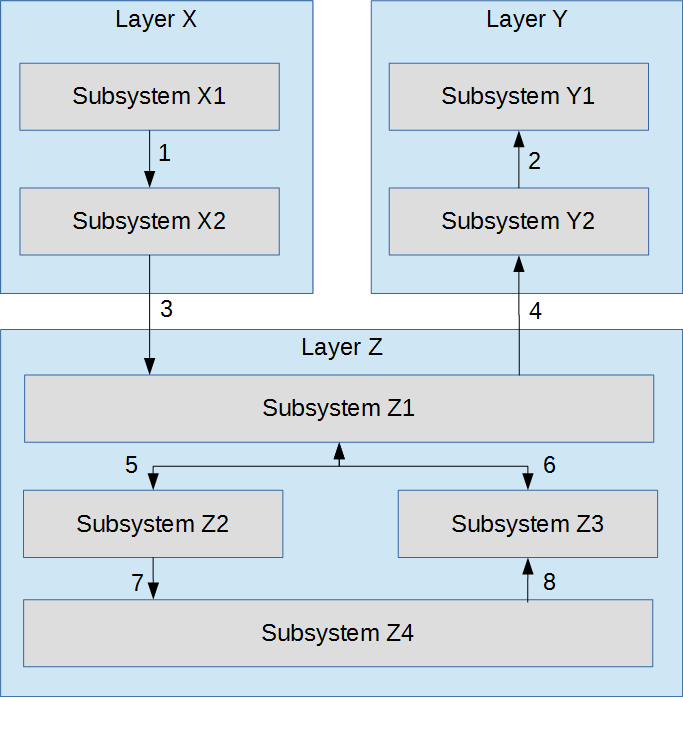
\includegraphics[width=0.90\textwidth]{images/data_flow}
 \caption{System architecture}
\end{figure}

\section{Roles \& Responsibilities}
% Each of us tal about what we are good at based on what we ae taking responsibilitiy for within the rover project. Point of contect for sponser we will just say conly is our sponser  so who in our team is our point of contect? Raya is currently scrm master right? but we agreed it would swap around?? Who are stakeholders. we hold stake right? university for paying for it? !!!!!
% 4316_Fa24_TR11_Project_Charter.mp4 time 20:50

As of now, Raya Sultan is assigned as the SCRUM master, and () is our product owner. These are subject to change over time. Our point of contact from the sponsor side will be Christopher Conly, from the team side it is Andrew Howard. At present, the university is the stakeholder of the project, given it is an educational project to aid other students in their real-time understanding of different navigation algorithms. Our sponsor is Christopher Conly.

Abubakar Kassim, due to his experience in software engineering, is responsible for programming and simulating various navigation algorithms. 

Madison Gage, due to her experience building an indoor rover, focus on designing and assembling the indoor rover.

Christopher Davis, due to his experience with embedded systems will focus on designing and assembling the indoor rover.

Raya Sultan, due to her graphics as well as engineering skills, will focus on drawing up schematics and diagrams, as well as assist in assembling the motor.

Andrew Howard, with his experience in digital systems, will focus on interfacing the hardware of the indoor rover with abstract software.

%Who are the stakeholders of the project? Who will be the point of contact from the sponsor or customer side? Who are the team members, and what will be their areas of responsibility? Will your team maintain the product owner and scrum master for the whole project, or will that role change periodically? This section should occupy 1/2 - 1 full page.
\newpage
\section{Cost Proposal}
This section contains the approximate budget for the project, where that money will come from, and any other support. The money will be provided by the University of Texas at Arlington CSE department. The circuit boards for a rover to function would cost over the amount the University is providing so we will be reusing boards that were part of previous rovers which would be used to cut down on overall cost. 
%This text should be replaced with a discussion and justification of major expenses, but not the actual monetary amounts (that will go in the preliminary budget section below). 

\subsection{Preliminary Budget}
\begin{itemize}
  \item Any circuit components that needs to be replaced.
  \item 3D printing components to add onto the rover
  \item Software licensees for navigational systems
\end{itemize}
%Include a high level budget table for components, fabrication, software licensees, development hardware, etc. This should be in a tabular format broken up into appropriate line items. 

\subsection{Current \& Pending Support}
University of Texas at Arlington CSE department is funding our project with \$800. 
%What are all of the funding sources for the project, and are there any potential funding sources that haven't been secured yet? List all funding sources (including the default funding amount provided by the CSE department) and their dollar amounts.
\section{Facilities \& Equipment}
Our team will need lab space in order to work on our rover. We will also need access to a rover/drone cage for safe testing of the rover. This testing ground is already present in the senior design labs we are provided.

We will require hardware components necessary for building an indoor navigation rover. This includes and is not limited to processors, power supplies and sensors. Furthermore, our team needs a place to store our rover, components, and related tools. There are black bins located in the senior design labs already that can be reserved, which covers tools and components. However, the rover is too large to be stored in the bin.

Already present in the lab are the retired UTARI rovers. This provides our team with a lot of starting materials. The rover will still require some components we do not have and these we will have to be purchase. Cannibalizing the UTARI rover and assembling the new rover will require tools, such as screwdrivers, wire cutters, soldering iron, wires, and more. Most of these tools are available to us in the senior design labs. Our team might need access to a MakerSpace to 3D print parts to hold or support components inside the rover. Further needs and and other equipment will be put here.

%What lab space, testing grounds, makerspaces, etc. will you need to complete the project? Will you require any specific equipment, and if so, where will you get it (borrow, lease, purchase, outsource, already present in the lab, etc.). This section should occupy 1/2 page.
\section{Assumptions}
%An assumption is a belief of what you assume to be true in the future. You make assumptions based on your knowledge, experience or the information available on hand. These are anticipated events or circumstances that are expected to occur during your project's life cycle.

%Assumptions are supposed to be true but do not necessarily end up being true. Sometimes they may turn out to be false, which can affect your project significantly. They add risks to the project because they may or may not be true. For example, if you are working on an outdoor unmanned vehicle, are you assuming that testing space will be available when needed? Are you relying on an external team or contractor to provide a certain subsystem on time? If you are working at a customer facility or deploying on their computing infrastructure, are you assuming you will be granted physical access or network credentials?

%This section should contain a list of at least 5 of the most critical assumptions related to your project. For example:

The following list contains critical assumptions related to the implementation and testing of the project.

%%%%%%%%%%%%%%%%%%%%%%%%%%%%%%%%%%%%%%%%%%%%%%%%%%%%%%%%%%%%%%%%%%%%%%%%%
% This creates a bullet list. To add a bullet, use the \item command.
% Make sure it is between the \begin{itemize} and \end{itemize} commands.

% The indentation of the items is optional and is for code readability.
\begin{itemize}
  \item Getting the rover to move in one direction by the 2nd sprint cycle
  \item A path finding system developed by the team coders will be done by the 4th sprint cycle
  \item Controlling the direction of the rover will be done by the 4th sprint cycle
  \item Testing the path finding system with the rover indoors will be done in the 4th sprint cycle
  \item Adding different parts that can be attached will be done after the 4th sprint cycle.
\end{itemize}
\section{Constraints}
%Constraints are limitations imposed on the project, such as the limitation of cost, schedule, or resources, and you have to work within the boundaries restricted by these constraints. All projects have constraints, which are defined and identified at the beginning of the project.

%Constraints are outside of your control. They are imposed upon you by your client, organization, government regulations, availability of resources, etc. Occasionally, identified constraints turn out to be false. This is often beneficial to the development team, since it removes items that could potentially affect progress.

%This section should contain a list of at least 5 of the most critical constraints related to your project. For example:

The following list contains key constraints related to the implementation and testing of the project.

%%%%%%%%%%%%%%%%%%%%%%%%%%%%%%%%%%%%%%%%%%%%%%%%%%%%%%%%%%%%%%%%%%%%%%%%%
% This creates a bullet list. To add a bullet, use the \item command.
% Make sure it is between the \begin{itemize} and \end{itemize} commands.
% The indentation of the items is optional and is for code readability.
\begin{itemize}
  \item The base robot was not initially designed by our team.
  \item Limited to certain components that would be out of budget to replace.
  \item Limited range of motion due to design of robot wheels.
  \item Total development costs must not exceed \$800.
  \item Limited to the sensors, such as limited to the range of the LiDAR.
\end{itemize}

\section{Risks}
This section lists 5 of the most critical identified risks that may hamper the progress and success of the project. Mitigation strategies will be discussed further in future meetings.


%%%%%%%%%%%%%%%%%%%%%%%%%%%%%%%%%%%%%%%%%%%%%%%%%%%%%%%%%%%%%%%
% This is the table. To add a row, separate each column with an
% ampersand (&) and end the line with the \hline command.
\begin{table}[h]
\resizebox{\textwidth}{!}{
\begin{tabular}{|l|l|l|l|}
\hline
 \textbf{Risk description} & \textbf{Probability} & \textbf{Loss (days)} & \textbf{Exposure (days)} \\ \hline
 Vital components being proprietary  & 0.25 & 5 & 1.25 \\ \hline
 The retired rover not being salvageable  & 0.20 & 14 & 2.8 \\ \hline
 The rover being damaged in transport & 0.30 & 10 & 3 \\ \hline
 Delays in shipping from overseas vendors  & 0.10 & 20 & 2.0 \\ \hline
 Reordering damaged components  & 0.10 & 10 & 2.0 \\ \hline
\end{tabular}}
\caption{Overview of highest exposure project risks} 
\end{table}
\section{Documentation \& Reporting}
%%% In this section, you will describe all of the various artifacts that you will generate and maintain during the project life cycle. Describe the purpose of each item below, how the content will be generated, where it will be stored, how often it will be updated, etc. Replace the default text for each section with your own description. Reword this paragraph as appropriate.

\subsection{Major Documentation Deliverables}

\subsubsection{Project Charter}
This document will be updated once every week, unless any major change or update occurs. The initial document is set to be submitted on 10/09/2024, Wednesday, and the final document is to be submitted in April 2025.
%Describe how this document will be maintained and updated (how often, under what circumstances, etc.). When will the initial version be delivered? When will the final version be delivered?

\subsubsection{System Requirements Specification}
This document will be updated once every week, unless any major change or update occurs. The initial document is set to be submitted on 10/09/2024, Friday, and the final document is to be submitted in April 2025.
%Describe how this document will be maintained and updated (how often, under what circumstances, etc.). When will the initial version be delivered? When will the final version be delivered?

%\subsubsection{Architectural Design Specification}
%Describe how this document will be maintained and updated (how often, under what circumstances, etc.). When will the initial version be delivered? When will the final version be delivered?

\subsubsection{Detailed Design Specification}
This document will be updated weekly based on progress with the rover and the navigation system. The initial version will be delivered on 10/09/2024 and the final document is to be submitted in April 2025.
%Describe how this document will be maintained and updated (how often, under what circumstances, etc.). When will the initial version be delivered? When will the final version be delivered?

\subsection{Recurring Sprint Items}

\subsubsection{Product Backlog}
The product backlog will be decided as a group vote and will prioritized based on how important it is toward goal of having a educational robot. Github will be used to share the code for the rover. Overleaf and Discord will be used to discuss the rest of what is needed for the rover to function.
%How will items be added to the product backlog from the SRS? How will these items be prioritized? Who makes the decision (product owner, group vote, etc.)? What software will be used to maintain and share the product backlog with team members and stakeholders?

\subsubsection{Sprint Planning}
There will be 9 sprints. Each sprint will be planned based on sprint backlog items and future goals for the rover.
%How will each sprint plan be planned? How many sprints will there be (you need to look at the schedules for this course and previous Senior Design II courses during the appropriate semesters to figure this out).

\subsubsection{Sprint Goal}
The sprint goal will be decided by the group and be discussed as the rover gets built.
%Who decides the sprint goal? How will you involve your customer in this process?

\subsubsection{Sprint Backlog}
The sprint backlog will be decided as a group and will be organized with hardware task and software task. We use github to collaborate on the software and use overleaf and discord to discuss what hardware to focus on.
%Who decides which product backlog items make their way into the sprint backlog? How will the backlog be maintained (collaboration software, a "scrum board", etc.)?

\subsubsection{Task Breakdown}
Tasks will be assigned to team member who volunteer and for the task that are not picked will be given to the members that have enough time and willing to take on the task.
%How will individual tasks be assigned from the sprint backlog? Will it be up to each team member to voluntarily claim a task, or will it come from the product owner? How will time spent on tasks be documented?

%%%%%%%%%%%%%%%%%%%%%%%%%%%%%%%%%%%%%%%%%%%%%%%%%%%%%%%%%%

% \subsubsection{Sprint Burn Down Charts} (REMOVED)
% Who will be responsible for generating the burn down charts for each sprint? How will they be able to access the total amount of effort expended by each individual team member? What format will the burn down chart use (include an example burn down chart below).

%  Be sure to update the image caption (REMOVED)
% \begin{figure}[h!]
%    \centering
%    
\includegraphics[width=0.5\textwidth]{images/test_image} % Image with a width of half of the text width
%    \caption{Example sprint burn down chart} % Caption - it automatically numbers the figures
% \end{figure}

%%%%%%%%%%%%%%%%%%%%%%%%%%%%%%%%%%%%%%%%%%%%%%%%%%%%%%%%%%

\subsubsection{Sprint Retrospective}
The sprint retrospective will be due on 10/21/2024. We as a team will discuss this after each week on Friday to pull all of our information.
%How will the sprint retrospective be handled as a team? When will this discussion happen after each sprint? What will be documented as a group and as individuals, and when will it be due?

\subsubsection{Individual Status Reports}
Each member will submit a report about their perspective about how the project is going and how each member is contributing. This will be reported after every sprint.
%What sort of status will be reported by each individual member, and how often will it be reported? What key items will be contained in the report?

\subsubsection{Engineering Notebooks}
The engineering notebook will be updated each week by each team member when they are in lab and at the end of each sprint each member would have to have an entry in the notebook. The minimum amount of pages per sprint would be 5 pages. Professor Conly will be the witness for each ENB page. Each member will be held accountable for their own entry.
%How often will the engineering notebook be updated, at a minimum, by each team member? What is the minimum amount of pages that will be completed for each interval, and how long will that interval be? How will the team keep each member accountable? Who will sign of as a "witness" for each ENB page?

\subsection{Closeout Materials}

\subsubsection{System Prototype}
The final system prototype will include a navigation system as well as different components like a pushy arm, sensors and a speaker. The rover will be demonstrated at the end of the spring semester.
%What will be included in the final system prototype? How and when will this be demonstrated? Will there be a Prototype Acceptance Test (PAT) with your customer? Will anything be demonstrated off-site? If so, will there be a Field Acceptance Test (FAT)?

\subsubsection{Project Poster}
The poster will include the rover as well as the many different functions it can do. The dimensions will be 24x32 and will be done by the end of the 4th sprint.
%What will be included on the poster, what will be the final dimensions, and when will it be delivered?

\subsubsection{Web Page}
The project webpage will serve as a key communication tool, showcasing the evolution of our pathfinding algorithms through detailed simulation videos. These videos will demonstrate various versions of our algorithms in action, alongside comparisons to the physical model, providing a clear visualization of performance and accuracy. This will allow users to assess how well the algorithms perform in real-world scenarios and how they improve over time. The webpage will also include a GitHub link, granting access to the project's source code and version history, promoting transparency and enabling collaboration. It will be accessible to the public, allowing stakeholders, potential collaborators, and the wider community to engage with our progress.


\subsubsection{Demo Video}
The demo videos will cover a wide range of topics related to the rover. Such as the key components that allow for different navigation algorithms to be tested on the rover. How to program the rover and what languages are used to do so. The demo video will include b-reel of the rover in action demonstrating different navigation algorithms. Should ideally take around 3-5 mins.

%What will be shown in the demo video(s)? Will you include a B-reel footage for future video cuts? Approximately how long will the video(s) be, and what topics will be covered?

\subsubsection{Source Code}
Our source code will be maintained using GitHub. The project will be open-source under the GPL (GNU General Public License), as many of our pathfinding algorithms (A*, Djikstra, Depth First Search, etc.), are open-source software, to promote transparency.

By adopting the GPL public license, we ensure that the derivations of our source code are open source. The source code including the binaries, will be provided to the customer, to ensure full control over the implementation. The customer can locate the source code via Github, where they have direct access to the repository.  All information containing our licensing will be contained within a readme file at the root of the repository.

\subsubsection{Source Code Documentation}
For code documentation, we will primarily utilize GitHub to ensure version control and collaborative efficiency. In addition, we will use Overleaf for generating our project documentation, which will be published as a downloadable PDF for easy access and distribution. 

\subsubsection{Hardware Schematics}
We will be documenting the connections between the PCB, Sabertooth motor drivers, DC converters, Signal Controllers, and any other component that is added in future sprints.
%Will you be creating printed circuit boards (PCBs) or wiring components together? If so, list each applicable schematic and what sort of data it will contain (PCB layout, wiring diagram, etc.). If your project is purely software, omit this section.

\subsubsection{CAD files}
We plan to use 3D printed parts to add on to the rover. We would be using Blender, Plasticity, or any of the available 3D modeling software.
%Will the project involve any mechanical design, such as 3D printed or laser-cut parts? If so, what software will you use to generate the files and what file formats will you provide in your closeout materials (STL, STEP, OBJ, etc.). If your project is purely software, omit this section.

\subsubsection{Installation Scripts}
The customer will be able to deploy their own navigation system through flashing onto the device by connecting it to the main board. We will provide a basic navigation system to demo the rover's capabilities.
%How will the customer deploy software to new installations? Will you provide installation scripts, install programs, or any other tools to improve the process? Will there be multiple scripts provided (perhaps separate scripts for the graphical front end and back end server software)? 

\subsubsection{ User Manual}
The customer would either need a digital user manual or a physical copy to understand what buttons do what and where extra additions can be placed. 
%Will you customer need a printed or digital user manual? Will they need a setup video? Decide now what will be provided and discuss.

\newpage

%%% References
%\bibliographystyle{plain}
\bibliographystyle{reference/IEEEtran_custom}
\bibliography{reference/refs}{}

\end{document}